\documentclass[twoside,a4paper,titlepage,11pt]{report}

\usepackage[utf8]{inputenc}
\usepackage[a4paper, total={6in, 8in},headheight=14pt]{geometry}
\usepackage{newtxtext,newtxmath}
\usepackage[scaled=1]{couriers}
\usepackage[spanish]{babel}
\usepackage{microtype}
\usepackage[bottom]{footmisc}
\usepackage{fancyhdr}
\usepackage{graphicx}
\usepackage{blindtext}
\usepackage{scrextend}
\usepackage{tocloft}
\usepackage{parskip}
\usepackage{multicol}
\usepackage{subcaption}
\usepackage{wrapfig}
\usepackage{multicol}
\usepackage{verbatimbox}
\usepackage[nottoc, notlot, notlof]{tocbibind}
\usepackage{listingsutf8}
\usepackage{url}
\usepackage[square,numbers]{natbib}
\usepackage{adjustbox}
\usepackage[makeroom]{cancel}
\usepackage[hidelinks]{hyperref}
\usepackage[Glenn]{fncychap}
\usepackage{lastpage}
\usepackage{fancyhdr}

\bibliographystyle{unsrtnat}

\pagestyle{fancy}
\fancyhf{}
\fancyhead[R]{\rightmark}
\fancyfoot[C]{\leftmark}
\fancyfoot[R]{\thepage}
\renewcommand{\footrulewidth}{0.6pt}% Line at the footer visible
\addto\captionscatalan{%
  \renewcommand\contentsname{Índice}%
}

\fancypagestyle{plain}{%
  \fancyhf{}%
  \fancyfoot[R]{\thepage}%
  \renewcommand{\headrulewidth}{0pt}% Line at the header invisible
  \renewcommand{\footrulewidth}{0.6pt}% Line at the footer visible
}


\renewcommand{\cftpartleader}{\cftdotfill{\cftdotsep}}%
\renewcommand{\cftsecleader}{\cftdotfill{\cftdotsep}}%
\renewcommand\familydefault{\sfdefault}

\usepackage{tikz}
\usetikzlibrary{shapes.geometric, arrows}

\newcommand{\Lagr}{\mathcal{L}}
\newcommand{\Xagr}{\mathcal{X}}

\setlength{\skip\footins}{1cm}

\makeatletter
% \patchcmd{<cmd>}{<search>}{<replace>}{<success>}{<failure>}
\patchcmd{\@makechapterhead}{\huge}{\large}{}{}% for \chapter
\patchcmd{\@makechapterhead}{\Huge}{\large}{}{}% for \chapter
\patchcmd{\@makeschapterhead}{\Huge}{\large}{}{}% for \chapter*
\makeatother


\begin{document}

\iftrue
\newcommand{\HRule}{\rule{\linewidth}{0.5mm}}

\thispagestyle{empty}

\begin{center}

{\large Universitat Politècnica de Catalunya}

\medskip
{\large Facultat d'Informàtica de Barcelona (FIB)}

\vfill
{\bfseries\Large Bachelor's Degree Project}

\vfill
\centerline{\mbox{
\includegraphics[width=60mm]{media/FIB_UPC.png}}}

\vfill
\vspace{5mm}

{\LARGE Jordi Gil González}

\vspace{15mm}

% Title in English according to the official assignment
{\LARGE\bfseries Analysis of the Path Tracing \\ rendering method on CPU and GPU}

\normalfont \small \sffamily{}

\vfill

Computer Science Department


\vfill

\begin{tabular}{rl}
Bachelor's Degree Project Director: & Chica Calaf, Antoni \\
\noalign{\vspace{2mm}}
Study programme: & Computer Science\\
\noalign{\vspace{2mm}}
Specialization: & Computer Graphics\\
\end{tabular}

\vfill

\large Academic Year 2019/2020

\large \today

\end{center}

\newpage
\tableofcontents*
\fi

\newpage

\chapter{Contextualización y alcance del proyecto}

\section{Introducción}

En la actualidad las imágenes generadas por ordenador están muy presentes en nuestro día a día, ya sea en un entorno de trabajo o en un lúdico. La creación de imágenes realistas mediante el uso de computadoras se ha convertido en una necesidad de actualidad. Industrias como el cine o los videojuegos requieren de algoritmos capaces de poder reproducir el mundo real en un entorno virtual en el menor tiempo posible.

El estudio de métodos que permiten renderizar imágenes realistas no es nuevo. Entre principios y mediados de los años 70 comenzaron a publicarse los primeros artículos científicos sobre iluminación realista. El sombreado Gouraud (\textit{Gouraud Shading}), el sombredado Phong (\textit{Phong Gouraud}) y el sombreado Blinn-Phong (\textit{Blinn-Phong Shading}) son ejemplo de ello. Estos algoritmos tienen en cuenta solamente la luz ambiente, la luz difusa y la luz especular. 

\begin{figure}[ht]
	\centering
	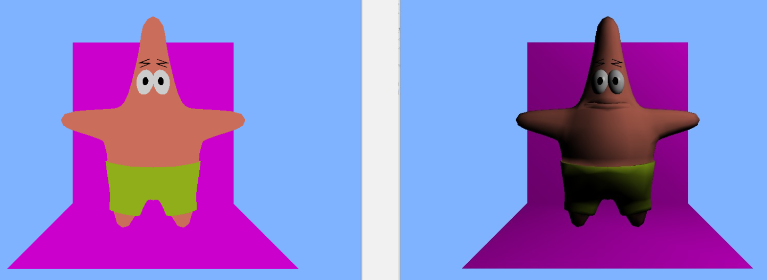
\includegraphics[scale=0.5]{media/shading_idi.png}
	\caption{}
    \label{fig:idi}
\end{figure}

En computación gráfica existe un conjunto de métodos que nos permiten generar imágenes realistas: \textit{Ray Tracing} \cite{Whitted1980}, \textit{Path Tracing} \cite{Kajiya1986}, \textit{Bidirectional Path Tracing} \cite{Lafortune1993}, \textit{Photon Mapping} \cite{Jensen1996}, \textit{Metropolis light Transport} \cite{Veach1997}, entre otros. A excepción del \textit{Ray Tracing}, el resto de métodos listados tratan de aproximar la \textit{Rendering Equation} presentada por Kajiya et al. \cite{Kajiya1986}.



En éste proyecto nos centraremos en la implementación del \textit{Path Tracing} presentada por \cite{Shirley2018a} en su libro.

Nos planteamos tres grandes objetivos:

\begin{enumerate}
	\item \label{a} Búsqueda de información sobre técnicas de optimización usadas en éste tipo de métodos
	\item Implementación para CPU y GPU de les técnicas vistas en el punto \ref{a}
	\item Análisis y comparación de los resultados obtenidos en ambas implementaciones.
\end{enumerate}

\section{Contextualización}

\subsection{Contexto}

La renderización de imágenes realistas es un área de gran interés en el campo de la computación gráfica. Un de los principales objetivos de ésta, es ser capaces de renderizar imágenes que sean indistinguibles de las del mundo real, como por ejemplo fotografías. Es por eso, que es muy importante poder reproducir el comportamiento de la luz en un entorno virtual. Para poder obtener este realismo es necesario la iluminación global, es decir, hemos de ser capaces de poder simular la luz directa (luz que incide de forma directa a un objeto de la escena desde el foco de luz) i la luz indirecta (luz que incide a un objeto de los rebotes en otros objetos de la escena).

El algoritmo de \textit{Ray Tracing} es un de los métodos más populares de este conjunt. Se trata de una técnica que consiste en trazar rayos desd el foco de luz (\textit{Forward Ray Tracing}) a los diferentes objetos de la escena, o des de el ojo, o cáaera virtual, (\textit{Backward Ray Tracing}). Éste es muy sensible al nombre de polígonos que contiene las escena, a más compleja es más infeciente será. Todo y proporcionarnos un alt grado de realismo, no es capaz de conseguir un efecto foto-realista debido a no tener en cuenta la iluminación indirecta. Para conseguir este efecte, hemos de tener presente tanto la iluminación directa com la indirecta, es por eso que Kajiya et al. presentó la \textit{Rendering Equation} \cite{Kajiya1986}. A pesar de tener ciertas limitaciones y no representar todos los efectos que la luz produce en el mundo real como por ejemplo el \textit{Subsurface Scattering}, un método que aproxime esta ecuación ya nos permitirá renderizar imágenes foto-realistas.

El algoritmo de \textit{Path Tracing} surge como mejora del \textit{Ray Tracing} con el objetivo de dar una solución a la \textit{Rendering Equation} mediante la integración de Monte Carlo. Gracias a ésto, el algoritmo es capaz, de forma natural, representar efectos como \textit{Motion Blur}, \textit{Ambient Oclussion} e iluminación indirecta sin necesidad de uso de shaders a posterior. En el \textit{Path Tracing} es indiferente el número de polígonos que conforman una escena, pero su mayor desventaja es el ruido. Se necesitan muchas muestras por cada píxel de la imagen para que la imagen converja, es por eso que resulta un algoritmo muy costoso para aplicaciones en tiempo real como videojuegos. En cambio, se lleva utilizando muchos años en industrias como el cine de animación dónde el tiempo de procesado de un frame no es tan importante en comparación a la calidad de imagen deseada.

Debido a que cada píxel es independiente de los demás, tenemos un algoritmo con una alta capacidad de paralelismo. Gracias a ésto, podemos explotar la capacidad que tiene la CPU y la GPU para ejecutar aplicaciones en paralelo y calcular más de un píxel al mismo tiempo. 


\subsection{Stakeholders}

En esta sección presentaremos los diferentes actores implicados en un proyecto.

\subsubsection{Desarrollador}

Este actor es el encargada de realizar la planificación del proyecto, búsqueda de información, documentación, desarrollo del software requerido, solución de posibles obstáculos y/o problemas que puedan aparecer a lo largo del desarrollo y realización y análisis de los experimentos. Debe trabajar de forma conjunta y coordinada con el director, y co-director i/o ponente en caso de haber, y es la última persona encargada del cumplimiento de los términos establecidos.

\subsubsection{Director del proyecto}

Este acto es el encargada de guiar al desarrollador en caso de dificultades, así como del asesoramiento de posibles soluciones.

\subsubsection{Usuarios beneficiados}

Aunque este proyecto no tiene la intención de crear un producto, no quiere decir que no existan beneficiarios. Explorar diferentes vías de optimización haciendo uso de arquitecturas paralelas puede ser útil para investigadores y desarrolladores en el campo de la computación gráfica.

\section{Justificación}

En la actualidad son muchas las librerías orientadas a la programación en GPU. Tenemos librerías como \texttt{OpenCL} u \texttt{OpenACC} que nos permiten una mayor portabilidad entre tarjetas gráficas de distintos fabricantes como por ejemplo \texttt{AMD} y \texttt{NVIDIA}. Pero para este proyecto hemos decidido escoger la API \texttt{CUDA} implementada por \texttt{NVIDIA} específicamente para sus tarjetas gráficas y aceleradores. Decidimos usar esta API debido a que al ser sotfware propietario de \texttt{NVIDIA} éste está mejor optimizado para las tarjetas de dicha empresa, que son las que utilizaremos en este proyecto.

Es posible que al comentar que usaremos tarjetas/aceleradores \texttt{NVIDIA} y el proyecto está enfocado al tema de renderizado de gráficos realistas nos venga a la mente la nueva gama de tarjetas RTX. En un inicio se planteó guiar el proyecto hacia el uso de tarjetas con tecnología RTX debido a que han sido diseñadas específicamente para el uso de \textit{Ray Tracing} en tiempo real. Esta idea fue descartada en seguida debido al elevado precio de éstas, el rango de precios de las tarjetas de esta gama está entre los 350€ en los modelos más barato hasta los varios miles de euros en modelos destinados a entornos profesionales. Finalmente, se adquirió una tarjeta Nvidia RTX 280 Super de 8Gb de memoria, pero debido al corto periodo de tiempo de desarrollo no guiamos el proyecto a utilizar dicha tarjeta de forma exclusiva estudiando y poniendo en práctica las nuevas mejoras que otras tarjetas de gamas inferiores no incluyen (RT Cores, Tensor Cores, Mesh Shaders, etc.). Es por eso que esta tarjeta gráfica será usada para probar nuestra aplicación, pero no en un sentido exclusivo.

Como hemos comentado al inicio de esta sección, \texttt{CUDA} es un API que está muy bien optimizada para hardware de \texttt{NVIDIA}. Esto nos da un punto a favor debido a que el la aplicación que vamos a desarrollar será probada en diferentes entornos:

\begin{enumerate}
	\item Computador portátil - Lenovo Legion Y520 con Nvidia GTX1050 - 4GB 
	\item Cluster docencia BOADA - 4 GPUs Nvidia Tesla K40c
	\item Computador personal - Nvidia RTX 2080 Super - 8Gb 
\end{enumerate}

Al usar tarjetas en entornos diferentes podremos analizar como nuestra aplicación responde en dichos entornos. Estudiar como es el rendimiento cuando utilizamos 4 tarjetas pensadas para un entorno de investigación en contra posición con dos tarjetas gráficas pensadas para el uso cotidiano. También podremos ver como es el rendimiento en una tarjeta gráfica de gama media (Nvidia GTX1050) y un gráfica de gama alta (Nvidia RTX 2080 Super).

\section{Alcance del proyecto}

Para solucionar el problema presentado en nuestro proyecto necesitamos una aplicación que sea capaz de renderizar imágenes realistas. En \cite{Shirley2018a}, \cite{Shirley2018b} i \cite{Shirley2018c} se presentan las bases para crear un \textit{Path Tracing}. A partir de esta base extenderemos nuestra aplicación a una versión paralela haciendo uso de la CPU y otra haciendo uso de la GPU. Se hará uso de diferentes técnicas de optimización comúnmente utilizadas en este tipo de aplicaciones, como por ejemplo el uso de estructuras de datos aceleradoras \cite{Hunt2008} para representar la escena de forma interna. En concreto, la estructura de datos que utilizaremos para genera la escena se trata de una \textit{Bounding Volume Hierarchy}, que se trata de una estructura de tipo árbol, ya sea binario o n-ario, donde cada hoja representa la caja englobante (\textit{Bounding Box}) de cada primitiva que existe en la escena, y cada nodo intermedio representa la caja englobante de sus hijos.

\subsection{Alcance}

En este apartado se presentan los diferentes objetivos y posibles obstáculos del proyecto.

\subsection{Objetivo}

El objetivo principal de este proyecto es desarrollar una aplicación que dada un escena, la renderice mediante \textit{Path Tracing} y analizar el rendimiento que éste nos da en su versión paralela en CPU y en GPU.

La gestión de memoria en una aplicación paralela, ya sea en CPU o en GPU, es muy importante y tener una mala gestión de ésta puede suponer que el rendimiento de nuestra aplicación no sea el esperado. Por eso definiremos como objetivo secundario, pero no menos importante, estudiar y llevar a cabo cuales son las mejores prácticas en este campo.

Como a sub-objetivos tenemos:

\begin{enumerate}
	\item Implementar de forma eficiente los algoritmos presentados en \citep{Shirley2018a} y \cite{Karras2012}
	\item Implementar de forma eficiente los cálculos de intersección rayo-objeto
\end{enumerate}

\subsection{Obstáculos i riesgos del proyecto}

Los temas principales que se tratan en el proyecto, como por ejemplo implementaciones del \textit{Path Tracing} o diferentes métodos de construcción de un BVH, están muy estudiados y desarrollados. No obstante, eso no implica que el desarrollo del proyecto sea un camino sencillo, son muchos los problemas a los cuales podemos enfrentarnos por el camino.

\subsubsection{Programa principal}

Como bien hemos comentado en la sección de objetivos, la gestión de memoria es un factor muy importante. Una mala gestión puede provocar errores en nuestra aplicación provocando que ésta no funcione correctamente o directamente no funcione.

\subsubsection{Algoritmo utilizado}

El algoritmo utilizado calcula el color a partir de la intersección de los rayos emitidos desde la cámara a los diferentes objetos de la escena. El cálculo de esta intersección debe ser muy eficiente ya que se trata de operaciones que se llevarán a cabo miles de millones de veces en la creación de una sola imagen. Tener una mala implementación puede afectar de manera negativa en el rendimiento de nuestra aplicación y en los experimentos a realizar.

\section{Metodología y rigor}

En esta sección veremos el conjunto de herramientas que se usaran a lo largo del desarrollo del proyecto. Para poder llevar un buen desarrollo de nuestro proyecto nos organizaremos de la siguiente forma. Cada 15 días habrá una reunión con el director para comentar el estado del proyecto, resultados obtenidos, carencias, objetivos cumplidos, no cumplidos y acordar los siguientes pasos a realizar. De cara a la fase final las reuniones serán semanales.

\subsection{Herramientas de desarrollo}

El desarrollo de nuestra aplicación se llevará a cabo en C++ haciendo uso de la librerías \texttt{OpenMP} y \texttt{CUDA}. 

\texttt{OpenMP} es una API diseñada para añadir concurrencia a programas escritos en \texttt{C}, \texttt{C++} y \texttt{Fortan}. La principal ventaja de usar esta API, en contra de otras de características similares, es que nos permite escribir un código portable entre diferentes sistemas operativos como Linux, Windows o MAC. Nos permite crear de forma sencillas aplicaciones paralelas haciendo uso de la CPU.

\texttt{CUDA} es una plataforma de computación paralela y una API desarrollada por \texttt{NVIDIA} y nos permite acceder al conjunto de instrucciones y elementos de las tarjetas gráficas de \texttt{NVIDIA}. Una gran ventaja de esta API es la gran accesibilidad, para usuarios novel, que tiene en contra de otras APIs orientadas a programación en GPU como por ejemplo \texttt{OpenGL}, \texttt{OpenCL} y \texttt{DirectX}.

\subsection{Herramientas de seguimiento}

Para poder llevar a cabo un buen seguimiento del desarrollo se hará uso de \texttt{git}. Esta herramienta nos permite llevar un control de versiones para poder acceder a versiones anteriores de nuestro código en caso de ser necesario.

\subsection{Validación de resultados}



\newpage

\bibliographystyle{ACM-Reference-Format}
\bibliography{./includes/library}

\end{document}
